
%%%%%%%%%%%%%%%% Nm Tutorial %%%%%%%%%%%%%%%%%%%%
\chapter{Netzwerk-Management Anleitung}
\label{sec:nm_tutorial}
% TODO:





%%%%%%%%%%%%%%%% VCAN-API %%%%%%%%%%%%%%%%%%%%
\chapter{VCAN-API}
\label{sec:vcan_api}
Dieses Kapitel beschreibt die im Laufe des Projektes erstellte Software zur Kommunikation per virtuellem CAN. Alle Informationen über das Protokoll wurden per Reverse Engineering ermittelt.
% TODO:


\section{Protokoll}
\label{sec:vcan_protokoll}
Das VCAN-Protokoll besteht aus einem Binär-Format, dass per TCP-Socket übertragen wird. Der Aufbau und Abbau der TCP-Verbindungen wird verwendet um Clients am Gateway an- und abzumelden. Zudem müssen Socket-Fehler abgefangen werden, da ein ordnungsgemäßer Verbindungsabbau nicht gegeben sein muss.

\begin{figure}[ht]
\centering
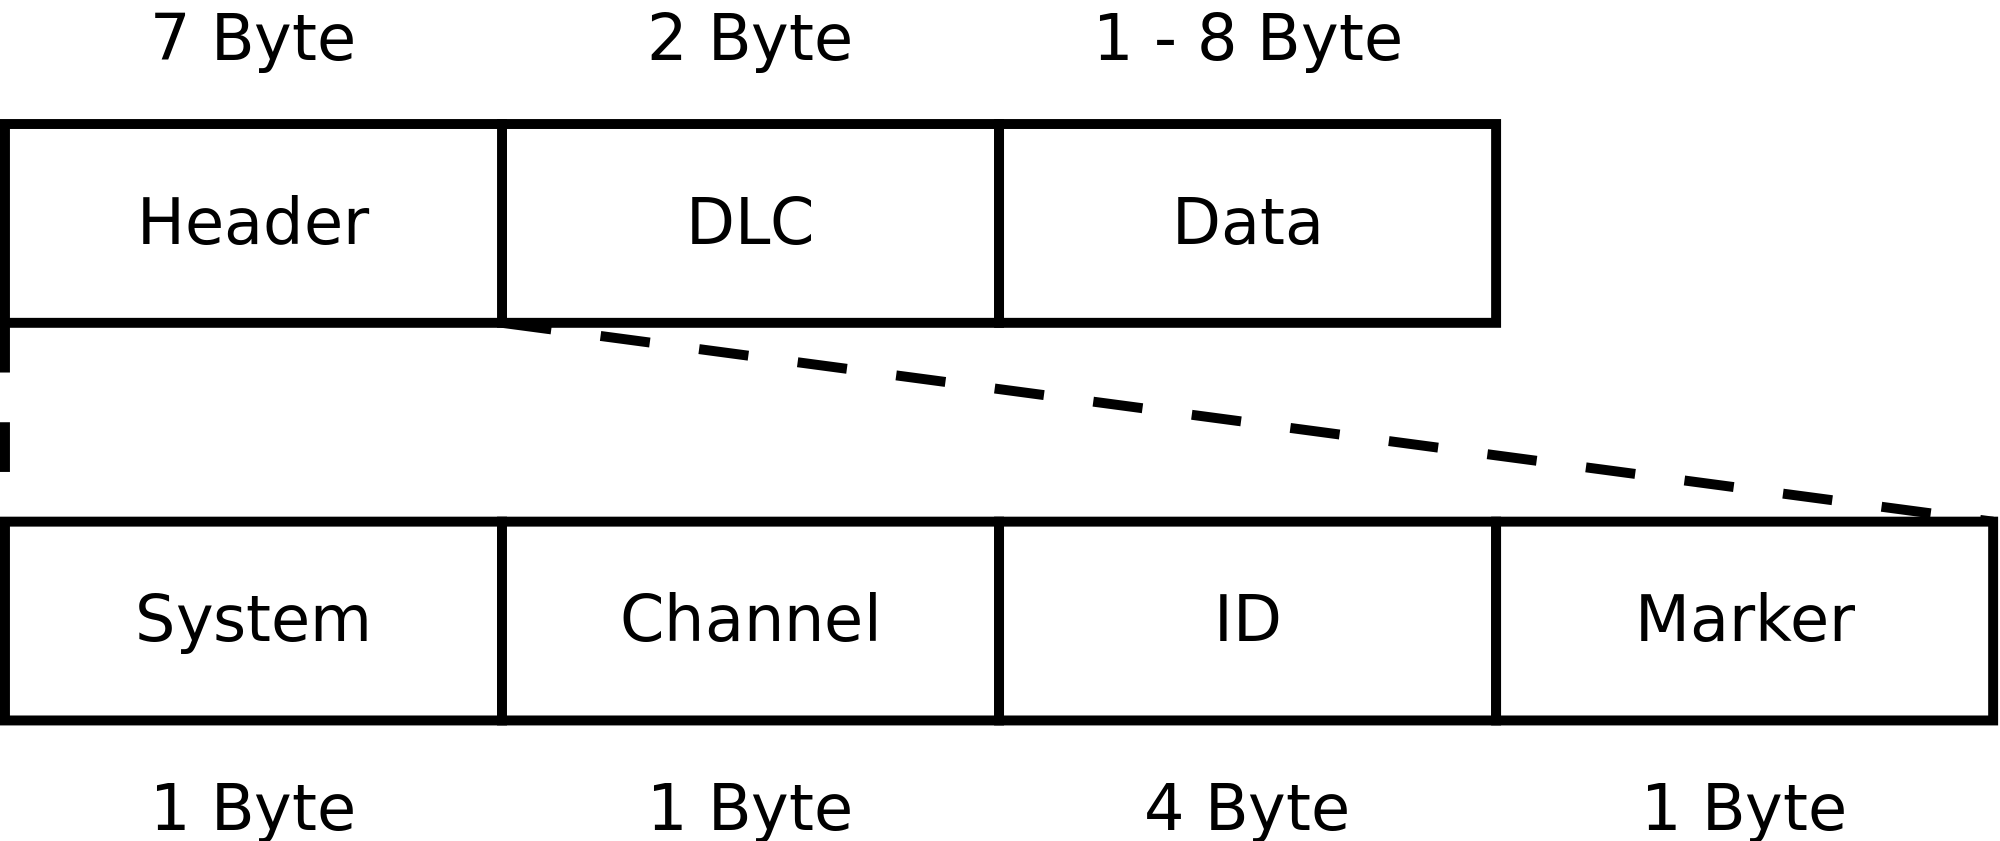
\includegraphics[width=0.8\textwidth]{vcan_protokoll}
\caption{Überblick über das VCAN Protkoll}
\label{fig:vcan_protokoll}
\end{figure}

Das eigentliche Binär-Format des Protokolls ist in Abbildung \ref{fig:vcan_protokoll} zu sehen. Das Format besteht aus einem Header, dem DLC-Feld und den eigentlichen Daten. Der Header enthält unter anderem die ID der Botschaft. Die Nutzdaten können 1 bis 8 Byte lang sein. Im folgenden ist eine ausfürliche Auflistung der Felder dargestellt. Die Byte-Reheinfolge entspricht Big-Endian. Tabelle \ref{tab:vcanbotschaft} zeigt eine Beispiel-Botschaft ohne TCP- und Ethernet-Header.

\begin{description}
    \item[System] \hfill \\ Angabe eines Systems (zum Beispiel CAN oder LIN). Eine Auflistung der möglichen Werte ist in Tabelle \ref{tab:vcansysteme} zu finden. Die symbolischen Namen stammen dabei aus dem Elektrobit Gateway
    \item[Channel] \hfill \\ Enthält eine Kanal-Nummer. Kann Werte von 0 bis 255 annehmen.
    \item[ID] \hfill \\ CAN-ID der Botschaft.
    \item[Marker] \hfill \\ Markiert extended CAN Frames. 0 steht für einen standard frame, jeder andere Wert für ein extendend Frame. Dies Byte könnte weitere Funktionalität bei LIN oder FlexRay Systemen haben.
    \item[DLC] \hfill \\ Anzahl der Daten-Bytes. Kann bei CAN nur Werte von 1 bis 8 annehmen. 
    \item[Data] \hfill \\ Nutzdaten. Die Anzahl der Bytes entspricht dem Wert im DLC-Feld.
\end{description}

\begin{table}[ht]
    \center
    \begin{tabular}[h]{c l}
        Hex Wert & Symbolischer Name \\
        \toprule
        0 & Unknown\\
        1 & Flexray1\\
        2 & Flexray2\\
        3 & CAN1\\
        4 & CAN2\\
        5 & CAN3\\
        6 & CAN4\\
        7 & LIN1\\
        8 & LIN2\\
        9 & bad allocation\\
        a & æI@\\
        b & <null>\\
        \bottomrule
    \end{tabular}
    \caption{Liste der VCAN Systeme}
    \label{tab:vcansysteme}
\end{table}

\begin{table}[ht]
    \center
    \begin{tabular}[h]{c l}
        Hex Wert & Bedeutung \\
        \toprule
        03 & System: CAN1\\
        \midrule
        00 & Channel: 0\\
        \midrule
        42 & \multirow{4}{*}{CAN-ID (hex): 742}\\
        07 & \\
        00 & \\
        00 & \\
        \midrule
        00 & Standard Frame\\
        \midrule
        04 & \multirow{2}{*}{DLC: 4 Bytes}\\
        00 & \\
        \midrule
        00 & \multirow{4}{*}{Daten: 00:00:2A:00}\\
        00 & \\
        2a & \\
        00 & \\
        \bottomrule
    \end{tabular}
    \caption{Beispiel VCAN Botschaft}
    \label{tab:vcanbotschaft}
\end{table}

Das Protokoll, wie es im Elektrobit-Gateway eingesetzt wird, hat einige Besonderheiten. So werden gelegentlich die Daten-Bytes mehrerer Botschaften angehängt. Hierbei wird der Header nur einmal, jedoch die Daten mehrerer Botschaften übermittelt. Auch wird zeitweise der Daten-Bereich einer Botschaft mehrfach angehängt. Das Verhalten konnte nicht zuverlässig nachvollzogen werden. Es hat jedoch den Anschein, dass diese Probleme durch eine hohe Netzwerk-Last beziehungsweise -Latenz hervorgerufen werden. Da nicht eindeutig eine Mehrfachsendung einer Botschaft von verschiedene Botschaften in einem Paket unterschieden werden kann, wurde dieses Verhalten nicht implementiert. 


\section{Projekt Struktur}
\label{sec:vcan_struktur}
% TODO:
% Abhängigkeiten

Im folgenden wird die Dateistruktur des Projektes näher betrachtet. Abbildung \ref{fig:vcan_api_uml} zeigt eine UML-Klassendiagramm der VCAN-API.

\begin{figure}[ht]
\centering
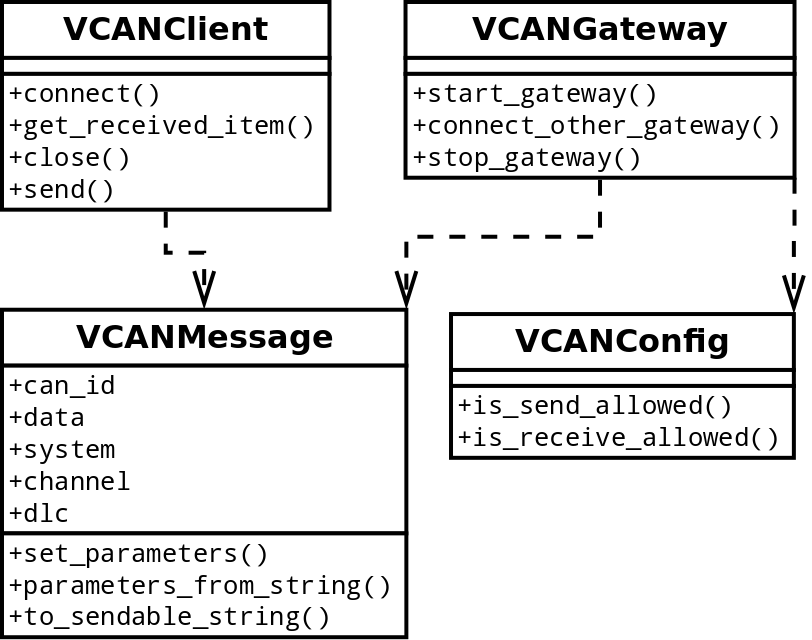
\includegraphics[width=0.8\textwidth]{vcan_api_uml}
\caption{UML-Klassendiagramm der VCAN-API}
\label{fig:vcan_api_uml}
\end{figure}

\begin{description}
    \apiitem{./vcan\_api/}
    Dieses Verzeichnis enthält die gesamte VCAN-API.
    \begin{description}
        \apiitem{./vcan\_api/\_\_init\_\_.py}
        VCAN-API Python Pyackage.
        \apiitem{./vcan\_api/PCANBasic.py}
        API zur Nutzung des PEAK-PCAN-USB-Adapters. Diese Datei stammt von PEAK.
        \apiitem{./vcan\_api/vcan\_client.py}
        Enthält die Klasse VCANClient.
        \apiitem{./vcan\_api/vcan\_config.py}
        Enthält die Klasse VCANConfig.
        \apiitem{./vcan\_api/vcan\_config.xsd}
        XML-Schema für Firewall-Konfigurationen.
        \apiitem{./vcan\_api/vcan\_exception.py}
        Enthält die Klasse VCANException.
        \apiitem{./vcan\_api/vcan\_gateway.py}
        Enthält die Klasse VCANGateway.
        \apiitem{./vcan\_api/vcan\_message.py}
        Enthält die Klasse VCANMessage und einige Konstanten um diese zu Nutzen.
    \end{description}
    % TODO
    \apiitem{./example\_client.py}
    Verschiedene Beispiele für die Implementierung eines VCAN-Clients.
    \apiitem{./example\_gateway.py}
    Verschiedene Beispiele für die Implementierung eines VCAN-Gateways.
    \apiitem{./gateway.py}
    Ein simples Gateway mit grafischer Oberfläche.
    \apiitem{./gateway\_rules.xml}
    Eine Beispiel-Konfiguration der im Gateway eingebauten Firewall-Regeln.
\end{description}


\section{Gateway API}
\label{sec:vcan_gateway_api}

% class VCANGateway
\begin{description}
    \apiitem{class VCANGateway(receive\_callback=None, connection\_callback=None)}
    Das Gateway nimmt Verbindungen von Clients entgegen und verteilt eingehende Botschaften an alle angemeldeten Clients weiter.
    \begin{description}
        \apiitem{start\_gateway(host='127.0.0.1', port=10020, rulesfile='')}
        Startet das Gateway auf IP \texttt{host} und dem Port \texttt{port}. Auf dem ausführenden Rechner muss ein Netzwerk-Interface mit der entsprechenden IP existieren. Der Port darf nicht durch eine andere Anwendung belegt sein. Optional kann eine Regeldatei angegeben werden um Firewall-Regeln zu definieren. Dies ist noch experimentell.
        \apiitem{stop\_gateway()}
        Stoppt das Gateway wieder. Anschließend kann mittels der \texttt{start\_gateway} Methode wieder gestartet werden. Es werden jedoch alle Verbindungen getrennt, und die Host IP muss ein weiteres mal angegeben werden.
        \apiitem{connect\_other\_gateway(host, port=10020)}
        Ein Gateway kann sich zu einem anderen Gateway verbinden um ein Netz zu bilden. Das Ziel-Gateway muss unter der IP \texttt{host} und dem Port \texttt{port} erreichbar sein. Diese Methode ist hilfreich, wenn zum Beispiel eine Firewall eingehende Verbindungen verbietet oder ein Gateway unter Linux mit einem Windows-Gateway verbunden wird, um den PCAN nutzen zu können.
        \apiitem{pcan\_init()}
        Initialisiert den ersten gefundenen PEAK-PCAN USB-Dongle mit einer Baud-Rate von 500kbaud. Das gwählte USB-Interface und die Baud-Rate können zur Zeit nur im Code geändert werden. PCAN Support ist im Moment nur unter Windows vorhanden und wird ansonsten durch eine VCANException markiert.
        \apiitem{pcan\_uninit()}
        Deinitialisiert den PEAK-PCAN USB-Dongle.
    \end{description}
\end{description}

% class VCANConfig
\begin{description}
    \apiitem{class VCANConfig(rulesfile)}
    Diese Klasse wird verwendet um Firewall-Regeln im Gateway zu implementieren. Hierzu wird eine XML-Datei mit Regeln übergeben. Diese Datei muss dem beiligenden Schema \texttt{vcan\_config.xsd} entsprechen. Das Gateway ist dafür verantwortlich die entsprechenden Überprüfungen beim Senden und Empfangen durchzuführen.
    \begin{description}
        \apiitem{is\_send\_allowed(ip, can\_id)}
        Überprüft ob die IP \texttt{ip} eine Botschaft mit der ID \texttt{can\_id} senden darf. Gibt True zurück falls erlaubt, und False falls verboten.
        \apiitem{is\_receive\_allowed(ip, can\_id)}
        Überprüft ob die IP \texttt{ip} eine Botschaft mit der ID \texttt{can\_id} empfangen darf. Gibt True zurück falls erlaubt, und False falls verboten.
    \end{description}
\end{description}

% class VCANException
\begin{description}
    \apiitem{class VCANException(value)}
    Exception der VCAN-API. Wird beim Gateway verwendet, falls die PCAN-Verbindung nicht initialisiert werden kann.
\end{description}




\section{Client API}
\label{sec:vcan_client_api}

% class VCANClient
\begin{description}
    \apiitem{class VCANClient(q\_length=1024)}
    Diese Klasse kann verwendet werden, um Zugriff auf den VCAN zu erhalten. Es bietet Funktionen um eine Verbindung aufzubauen und zu schließen. Außerdem können Botschaften empfangen und gesendet werden. Standardmäßig erfolgt das Empfangen auf Polling-Basis. Hierzu wird eine Queue der Länge \texttt{q\_length} angelegt. Der Anwender ist verantwortlich die eingehenden Daten häufig genug zu pollen. Alternativ kann für das Empfangen eine Callback-Funtion angegeben werden.
    \begin{description}
        \apiitem{connect(ip, port=10020, receive\_data=True, callback=None)}
        Verbindet den Client mit einem Gateway auf IP \texttt{ip} und Port \texttt{port}. Über den Schalter \texttt{receive\_data} kann das Empfangen von Botschaften deaktiviert werden. Der Parameter \texttt{callback} kann verwendent werden um eine Funktions-Referenz zu übergeben, die empfangene Botschaften direkt verarbeitet. Wirft \texttt{VCANException} falls keine Verbindung hergestellt werden kann.
        \apiitem{close(sleep\_time=0.5)}
        Schließt die aktuelle Verbindung. Der Parameter \texttt{sleep\_time} wird verwendet um nach dem Schließen der Verbindung einen Moment zu warten. Damit werden Eigenheiten des EB-Gateways und der AUTOSAR-Anwendungen ausgeglichen, da es ansonsten zu Fehlern kommen kann. Die Angabe erfolgt in Sekunden.
        \apiitem{get\_received\_item()}
        Gibt die älteste empfangene Botschaft zurück. Falls die Queue leer ist wird \texttt{None} zurückgegeben. Diese Methode muss im Polling-Betrieb häufig genug aufgerufen werden, um Daten-Verlust zu vermeiden.
        \apiitem{send(message, sleep\_time=0.2)}
        Sende die Botschaft \texttt{message} zum verbundenden Gateway. Die Botschaft kann sowohl als Binär-String, als auch als VCANMessage vorliegen. Der Parameter \texttt{sleep\_time} wird verwendet um Fehler zu vermeiden indem nach dem Senden ein Moment gewartet wird. Falls nur Applikation angebunden sind, die die VCAN-API nutzen kann dieser Wert auf 0 gesetzt werden. AUTOSAR-Applikation haben jedoch Probleme mit zu geringen Warte-Zeiten und können Botschaften verlieren oder sogar abstürzen. Die Angabe erfolgt in Sekunden. Falls der Client zu keinem Gateway verbunden ist, wird eine \texttt{VCANException} geworfer.
    \end{description}
\end{description}

% class VCANMessage
\begin{description}
    \apiitem{class VCANMessage()}
    Repräsentiert eine Botschaft in der VCAN-API. Der Konstruktur generiert eine leere Botschaft. Diese kann entweder über \texttt{set\_parameters()} von Hand mit Parametern gefüllt werden, oder über \texttt{parameters\_from\_string()} von einer eingehenden Nachricht aus einem Binär-String.
    \begin{description}
        \apiitem{set\_parameters(can\_id,  data, system, channel, dlc=None)}
        Setzt die Parameter der Nachricht entsprechend den Parametern. Parameter \texttt{can\_id} gibt die ID der Botschaft an. Die Nutzdaten sind werden in \texttt{data} erwartet und müssen als Liste übergeben werden. Die Parameter \texttt{system} und \texttt{channel} geben das entsprechende System und den Kanal an. Standard-Werte sind CAN und Kanal 0. Weitere Möglichkeiten sind in der Datei \texttt{vcan\_message.py} als Konstanten hinterlegt. Der letzte Parameter, \texttt{dlc}, gibt die Länge der Daten an. Falls \texttt{None} übergeben wird, wird die Länge des Daten-Arrays verwendet.
        \apiitem{parameters\_from\_string(m\_string)}
        Setzt die Parameter der Nachricht anhand des Binär-Strings \texttt{m\_string}. Diese entsprechen direkt dem TCP-Paket und können hierdurch in eine VCAN-API-konforme Form gebracht werden.
        \apiitem{to\_sendable\_string()}
        Wandelt die Botschaft in einen Binär-String um, der per TCP versendet werden kann.
    \end{description}
\end{description}

% class VCANException
\begin{description}
    \apiitem{class VCANException()}
    Exception der VCAN-API. Wird geworfen falls die Verbindung zu einem Gateway scheitert, oder eine Nachricht gesendet wird obwohl keine Verbindung besteht. Außerdem siehe \ref{sec:vcan_gateway_api}
\end{description}




\section{Beispiel Anwendungen}
\label{sec:vcan_beispiele}














